\documentclass[addpoints]{exam}

\usepackage{enumitem}
\usepackage{graphbox}
\usepackage{hyperref}
\usepackage{multirow}
\usepackage{tabularx}
\usepackage{tikz}
\usetikzlibrary{positioning}

\graphicspath{{images/}}


% Header and footer.
\pagestyle{headandfoot}
\runningheadrule
\runningfootrule
\runningheader{CS 440}{HW II: Foundations II}{Fall 2020}
\runningfooter{}{Page \thepage\ of \numpages}{}
\firstpageheader{}{}{}

\qformat{{\large\bf \thequestion. \thequestiontitle}\hfill[\totalpoints\ points]}
\boxedpoints

\title{Homework II: Foundations II}
\author{CS 440 Computer Graphics\\Habib University\\Fall 2020}
\date{Due: 18h on Friday, 25 September}

\begin{document}
\maketitle


Use \texttt{numpy.array} and related methods from \texttt{numpy} to cast and perform vector operations on \texttt{list} or \texttt{tuple} objects.

\begin{questions}
  
  %%%%%%%%%%%%%%%%%%%%%%%%%%%%%%%%%%%%%%%%%%%%%%%%%%
  \titledquestion{Line Drawing}[10]

  \noindent\begin{tabularx}{\linewidth}{lX}
    \includegraphics[align=t]{dda} &
    In the recitation, we drew lines with angles of 0$^\circ$, 45$^\circ$, and 90$^\circ$ to the horizontal. In this question we will extend line drawing to a line defined by any two arbitrary points using the \href{https://en.wikipedia.org/wiki/Digital_differential_analyzer_(graphics_algorithm)}{Discrete Differential Analyzer (DDA) algorithm}. In the figure, imagine the lower left endpoint to be $P, (x_1,y_1)$ and the upper right to be $Q, (x_2,y_2)$. The algortihm plots $P$ and then iteratively increments $x$ until $Q$ is reached.
  \end{tabularx}
  In each iteration, the value of $y$ is computed as the previous value plus a pre-computed value, $dy = \frac{y_2-y_1}{x_2-x_1}$, which is also called the \textit{gradient} or \textit{slope} of the line. For lines with a larger $y$-extent than $x$-extent, the roles of $x$ and $y$ are switched in the algorithm.
  
  \underline{Task}: Write a function, \texttt{draw\_line\_dda()} in the file \texttt{api.py}, that takes as arguments: a \texttt{MyImage} instance and a pair of points where each point is represented as a pair of \texttt{int} coordinates. The function writes the line between the two points to the image. Any color may be used.

  \underline{Testing}: Make sure to test your algorithm for edge cases. Some of these are
  \begin{itemize}
  \item a line of length 1, i.e. $P$ and $Q$ are the same,
  \item perfectly horizontal and vertical lines,
  \item a line of length 2, to ensure that both endpoints are drawn, and
  \item interchanging $P$ and $Q$ to ensure that the same line is drawn.
  \end{itemize}

  %%%%%%%%%%%%%%%%%%%%%%%%%%%%%%%%%%%%%%%%%%%%%%%%%%
  \titledquestion{Adding Color}[5]

  \noindent\begin{tabularx}{\linewidth}{lX}
    \includegraphics[align=t]{dda-color} &
    We will now assign color to the line endpoints and draw a line with a color gradient. The figure shows the same line as above but with a color gradient such that $P$ is red and $Q$ is green. Your function now not only interpolates the coordinates between $(x_1,y_1)$ and  $(x_2,y_2)$ but also the colors between $(r_1, g_1, b_1, a_1)$ and  $(r_2, g_2, b_2, a_2)$. The interpolation calculations are similar. This will be our default line drawing method.
  \end{tabularx}
  \underline{Task}: Write a function, \texttt{draw\_line()} in the file \texttt{api.py}, that takes as arguments: a \texttt{MyImage} instance, a pair of points, and a pair of colors. Each point is represented as a pair of \texttt{int} coordinates and each color as a 4-tuple of \texttt{int} values. The coordinate and color pairs are parallel, i.e. the color at index $i$ corresponds to the point at the same index. The resulting pixels are written to the image and returned as a \texttt{list}. Each entry in the \texttt{list} is a pair of the form: \texttt{(point, color)}.

  \underline{Testing}: Use similar tests as above to ensure that all colors, especially at both endpoints, are drawn.

  %%%%%%%%%%%%%%%%%%%%%%%%%%%%%%%%%%%%%%%%%%%%%%%%%%
  \titledquestion{Here Comes Poly}[5]

  \begin{center}
    \begin{tabular}{cc}
      \includegraphics[align=t]{tri} & \includegraphics[align=t]{quad}
    \end{tabular}
  \end{center}
  
  The next step is to draw polygons. Above are polygons with 3 (triangle) and 4 (quadrilateral) points. The vertices of the triangle are colored red, green, and blue. Those of the quad are assigned red, green, blue, and white.
  
  \underline{Task}: Write a function, \texttt{draw\_polygon\_dda()} in the file \texttt{api.py}, that takes as arguments: a \texttt{MyImage} instance, an $n$-tuple of points, and an $n$-tuple of colors. Each point is represented as a pair of \texttt{int} coordinates and each color as a 4-tuple of \texttt{int} values. The coordinate and color $n$-tuples are parallel, i.e. the color at index $i$ corresponds to the point at the same index. The resulting pixels are written to the image.

  \underline{Testing}: Test your function with various values of $n$, especially $n=1$. Make sure to \textit{close} the polygon, i.e. connect the last point with the first.

  %%%%%%%%%%%%%%%%%%%%%%%%%%%%%%%%%%%%%%%%%%%%%%%%%%
  \titledquestion{Fill it Up}[15]

  \begin{center}
    \begin{tabular}{cc}
      \includegraphics[align=t]{tri-fill} & \includegraphics[align=t]{quad-fill}
    \end{tabular}
  \end{center}

  We end our polygon journey with a \textit{filled} polygon. The above polygons are the same as in the previous questions, except that they are filled. For filling to work properly, the polygon must be \textit{convex}. There are various ways to define a convex polygon. We define a convex polygon as one which is the convex hull of its vertices. Both the above polygons are convex. Filling of non-convex polygons leads to undefined behavior.

  Filling is a basic task in computer graphics and there are various algorithms available. While you are free to use any algorithm of your choosing, one in line with our work in this assignment so far uses the following ideas. Think of each row of pixels as a \textit{scanline}. Draw the boundary (lines) of the polygon first and save the pixels and colors drawn. Specifically, for each scan line on which the pixels fall, save the x values and colors. Once all the boundary pixels are drawn, iterate over the scanlines, scan the points in each scanline by x-value and then draw lines between successive pairs of points. 
  Because the polygon is convex, we can be sure that the line we draw will only fill interior pixels in the polygon. Note that a check for convexity is not included so the passed polygon must define a convex polygon.

  This method will be our default for drawing polygons.

  \underline{Task}: Write a function, \texttt{draw\_polygon()} in the file \texttt{api.py}, that takes as arguments: a \texttt{MyImage} instance, an $n$-tuple of points, an $n$-tuple of colors, and an optional boolean variable that defaults to \texttt{True}. The function is similar to the one above except that it fills the drawn polygon when the boolean parameter is True and only draws the boundary otherwise.

  \underline{Testing}: Test your function with various color combinations.

  \newpage
  %%%%%%%%%%%%%%%%%%%%%%%%%%%%%%%%%%%%%%%%%%%%%%%%%%
  \titledquestion{Sierpinski Again}[10]
    \includegraphics[width=\linewidth]{sierpinski}\\
  We revisit the \href{https://en.wikipedia.org/wiki/Sierpinski_triangle}{Sierpinski triangle} and employ our triangle (polygon) drawing mechanism to construct it using ``Shrinking and duplication'' as follows.
  \begin{enumerate}
  \item Start with any triangle (triangle 1. top left).
  \item Shrink the triangle to $\frac{1}{2}$ height and $\frac{1}{2}$ width, make three copies, and position the three shrunken triangles so that each triangle touches the two other triangles at a corner (triangle 2. second from left). Note the emergence of the central hole.
  \item Repeat step 2 with each of the smaller triangles (triangle 3 and so on).
  \end{enumerate}

  \underline{Task}: Write a function, \texttt{sierpinski()} in the file \texttt{application.py}, that takes as argument an \texttt{int} value. The value specifies the level of recursion: 0 corresponds to the image 1, 1 to image 2, and so on. The function returns a \texttt{MyImage} instance containing all the triangles side by side as shown above. The dimensions of the image are just enough to accommodate the contained triangles. You may use any reasonable coloring and dimensions.

  \underline{Testing}: Test your image dimensions, make sure that a recursion level of 0 returns an image containing triangle 1 above.

  %%%%%%%%%%%%%%%%%%%%%%%%%%%%%%%%%%%%%%%%%%%%%%%%%%
  \titledquestion{The Smoothness Illusion: $\lim\limits_{n\rightarrow\infty} \diamond = \circ$}[10]
  \begin{center}
    \includegraphics[width=\linewidth]{circle}
  \end{center}

  \begin{tabularx}{\linewidth}{lX}

    \raisebox{-\totalheight}{
      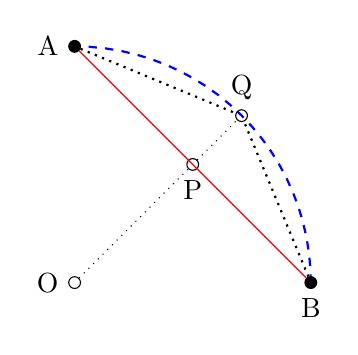
\begin{tikzpicture}
        \draw [blue,thick,dashed,domain=0:90] plot ({3*cos(\x)}, {3*sin(\x)});    
        \node [draw,circle,fill,inner sep=1.5pt,label=left:A] at (0,3) (a){};
        \node [draw,circle,fill,inner sep=1.5pt,label=below:B] at (3,0) (b){};
        \node [draw,circle,inner sep=1.5pt,label=left:O] at (0,0) (c){};
        \node [draw,circle,inner sep=1.5pt,label=below:P] at (1.5,1.5) (p){};
        \node [draw,circle,inner sep=1.5pt,label=above:Q] at (2.12,2.12) (q){};

        \draw [red] (a) -- (b);
        \draw [dotted] (c) -- (p);
        \draw [dotted] (p) -- (q);
        \draw [thick, dotted] (a) -- (q);
        \draw [thick, dotted] (b) -- (q);
      \end{tikzpicture}
    }
    &
    We draw a smooth surface on a discrete screen through approximation. That is, we display an approximation of the smooth surface which, with repeated subdivision, tends to the smooth surface. For example, a circle is approximated above by successively subdivided polygons. Each subdivision step inserts an edge midpoint at each egde and projects it to the circumference of the circle being approximated. This is illustrated in the figure on the left. The red edge AB approximates the blue arc AB of the circle centered at O. In the subdivision step, the midpoint, P, of the edge AB is projected to Q on the arc. The edge AB is then replaced by AQB.
  \end{tabularx}
  
  \underline{Task}: Write a function, \texttt{circle()} in the file \texttt{application.py}, that takes as argument two \texttt{int} values specifying the radius of the circle to be approximated and the number of subdivision steps to perform. No subdivision corresponds to the initial diamond only. The function returns a \texttt{MyImage} instance containing all the \textit{circles} side by side as shown above. The dimensions of the image are just enough to accommodate the contained circles. You may use any reasonable coloring and dimensions.

  \underline{Testing}: Test your image dimensions, make sure that a subdivision level of 0 returns an image containing yhe diamond above.

  %%%%%%%%%%%%%%%%%%%%%%%%%%%%%%%%%%%%%%%%%%%%%%%%%%
  \titledquestion{Mapping and Linear Interpolation}[0]
  \label{q:interpolate}

  \begin{tabularx}{\linewidth}{cX}
    \raisebox{-\totalheight}{
      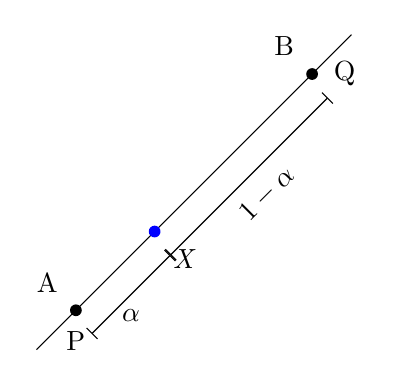
\begin{tikzpicture}
        \draw (0,0) -- (4,4);
        \node[circle,fill,inner sep=1.5pt] at (.5,.5) (P){};
        \node[circle,fill,inner sep=1.5pt] at (3.5,3.5) (Q) {};
        \node[circle,fill,blue,inner sep=1.5pt] at (1.5,1.5) (X) {};
        \node[below  = 2pt of P]{P};
        \node[right = 2pt of Q]{Q};
        \node[below right = 2pt of X]{\it X};
        \node[above left = 2pt of P]{A};
        \node[above left = 2pt of Q]{B};

        \draw[|-|] (0.7,0.2) -- node[midway,below=2pt]{$\alpha$}(1.7,1.2);
        \draw[|-|] (1.7,1.2) -- node[midway,sloped,below=2pt]{$1-\alpha$}(3.7,3.2);
      \end{tikzpicture}
    }
    &
    In the figure on the left, X lies on the line segment PQ such that
    \[
      |PX| : |XQ| = \alpha:(1-\alpha)\;,\; 0 \leq \alpha \leq 1,
    \]
    which leads to
    \[
      X = \alpha Q + (1-\alpha) P.
    \]
    That is, X is an affine combination of P and Q.
    
    Imagine a mapping from the range PQ to a new range AB. For example, P and Q may be vertices with colors A and B assigned to them respectively. We would be interested in finding out the color for X under this mapping. Generally, P, Q, and X belong to the same domain, and A and B are members of the same domain which may be different from the one that contains P, Q, and X.
  \end{tabularx}

  \underline{Task}: Write a function, \texttt{map\_point()} in the file \texttt{application.py}, that takes as argument, P, Q, A, B, and X. P, Q, and X belong to the same type. A and B belong to the same type. The function returns a value of the same type as A and B which is the mapping of X.

  \underline{Testing}: You can test this function against the \texttt{draw\_line()} function. Lines of the same length, slope, and vertex colors should have the same colors for intermediate pixels when drawn using \texttt{draw\_line()} and when assigned a color through this function.
  
  %%%%%%%%%%%%%%%%%%%%%%%%%%%%%%%%%%%%%%%%%%%%%%%%%% 
  \titledquestion{The Mandelbrot Set}[20]

  The sequence $z_n$ for a complex number, $c$, is defined for $n\geq 0$ as
  \[
    z_n(c) = \left\{
      \begin{array}{l@{\quad}l}
        0 & n = 0\\
        z^2_{n-1}(c)+c & \textrm{otherwise}
      \end{array}
    \right.
  \]

  \begin{figure}
    \centering
    \begin{tabular}{cc}
      \includegraphics[width=.47\linewidth]{mandelbrot1}& \includegraphics[width=.47\linewidth]{mandelbrot2}\\
      (a) & (b)
    \end{tabular}
    \label{fig:mandel}
    \caption{The Mandelbrot set up to $n_t = 100$. The points at the corners of the windows are outside the circle of radius 2, and $z_n$ escapes for these points at $n=1$. They are completely red. The points in blue toward the center of the image are the ones for which $z_n$ has not yet escaped. (a) Uniform color interpolation from Red to Green to Blue. (b) Adjusted color interpolation on the same data.}
  \end{figure}
  
The \href{http://en.wikipedia.org/wiki/Mandelbrot_set}{Mandelbrot set}, $M$, is the set of all complex numbers, $c$, for which $z_n(c)$ is \textit{bounded}, i.e. $|z_n|$ is finite for all $n$. It can be shown that if for some $n = n_0$, $|z_{n_0} > 2|$, then the sequence $z_n$ {\it escapes to infinity}, i.e. $|z_n|$ is not bounded for $n > n_0$. This leads to the conclusion that $\forall c \in M:\, z_n(c) \leq 2$. Since $z_1 = c$, the above condition also implies that $|c| \leq 2$.
The above yields the following two handy conditions whose fulfillment by a complex number, $c$, establishes its membership in $M$:
\begin{enumerate}
\item $|c|\leq 2$
\item $\forall n\geq 0:\, |z_n(c)|\leq 2$
\end{enumerate}
The value of $n$ for which condition 2 becomes false for a given $c$ is dubbed the {\it escape time} of $c$. Condition 2 also implies that all members of the Mandelbrot set lie within the circle in complex plane centered at the origin and with radius 2.

\underline{Example}: Consider the following complex numbers and the corresponding sequence for each up to $z_5$.
\[
  \begin{array}{c|*{4}{|c}}
 & c=(3+4j) & c=(1+1j) & c=(0.5+0.5j) & c=(-0.5-0.5j)\\\hline\hline
z_0(c) & 0 & 0 & 0 & 0\\
|z_0(c)| & 0 & 0 & 0 & 0\\\hline
z_1(c) & (3+4j) & (1+1j) & (0.5+0.5j) & (-0.5-0.5j)\\
|z_1(c)| & 5.0 & 1.41 & 0.71 & 0.71\\\hline
z_2(c) &  & (1+3j) & (0.5+1j) & (-0.5+0j)\\
|z_2(c)| &  & 3.16 & 1.12 & 0.5\\\hline
z_3(c) &  &  & (-0.25+1.5j) & (-0.25-0.5j)\\
|z_3(c)| &  &  & 1.52 & 0.56\\\hline
z_4(c) &  &  & (-1.69-0.25j) & (-0.69-0.25j)\\
|z_4(c)| &  &  & 1.71 & 0.73\\\hline
z_5(c) &  &  & (3.29+1.34j) & (-0.09-0.16j)\\
|z_5(c)| &  &  & 3.55 & 0.18\\\hline
  \end{array}
  \]

  \begin{itemize}
  \item We see that $z_1=c$. This follows from the definition of $z_n$.
  \item For the first number, $(3+4j)$, we see that $|z_1|>2$. We can therefore say that $z_n$ will escape to infinity and the escape time of $(3+4j)$ is 1. This expected as $(3+4j)$ lies outside the circle at the origin with radius 2.
  \item The second number, $(1+1j)$, lies within the required circle. But it escapes at n=2.
  \item The escape time for the third number, which is also inside the circle, is 5.
  \item The fourth number in also inside the circle and has not escaped until n=5. It may escape later or it may not. We cannot say.
  \end{itemize}
  
  \underline{Problem}: We want to visualize the Mandelbrot set up to a certain value of $n=n_t$ in an image. We will map our image to correspond to the circle in the complex plane which is centered at the origin and has a radius of 2. Each pixel in the image then corresponds to a complex number and is assigned a color corresponding to its escape time. In the figure above, complex numbers that escape early are assigned red and those that have not escaped till $n=n_t$ are assigned blue. Complex numbers with intermediate escape values are assigned interpolated colors. 

  Various steps are involved.
  \begin{enumerate}
\item Choose appropriate image dimensions and a value of $n_t$.
\item Map the x extent of our image to $[-2,2]$ on the real axis in the complex plane.
\item Map the y extent of our image to $[-2j,2j]$ on the imaginary axis in the complex plane.
\item Find the escape time of the complex number corresponding to each pixel in the image ans and assign a corresponding color to the pixel.
\end{enumerate}

  \underline{Task}: Write a function, \texttt{mandelbrot()} in the file \texttt{application.py}, that takes as argument an \texttt{int} value specifying $n_t$. It returns a \texttt{MyImage} instance containing a visualization of the Mandelbrot set up to $n=n_t$ as described above. The dimensions of the image are just enough to contain the discussed circle.

  \underline{Testing}: You will find that a simple linear interpolation between the colors for $n=1$ and $n=n_t$ will lead to a bland visualization as seen in Figure \ref{fig:mandel}a). You are encouraged to think about and implement an appropriate coloring scheme for the escape times. You may implement any coloring scheme that sufficiently distinguishes between different escape times.

  As you may imagine, this computation can be expensive. Pick an image resolution and $n_t$ that is feasible for your machine and which still leads to an interesting visualization.

  Make liberal use of the \texttt{map\_point()} function. Points 2, 3, and 4 above lend themselves simply to its use.

  You are encouraged to use the built-in \href{https://realpython.com/python-data-types/#complex-numbers}{complex data type} in python. Use of built-in Mandelbrot generators, e.g. \href{https://pillow.readthedocs.io/en/stable/reference/Image.html?highlight=mandelbrot#PIL.Image.effect_mandelbrot}{in Pillow} is forbidden.

\end{questions}

\end{document}
%%% Local Variables:
%%% mode: latex
%%% TeX-master: t
%%% End:
